\documentclass[journal,11pt]{IEEEtran}
\usepackage[utf8]{inputenc}
\usepackage{parskip}
\usepackage[sorting=none]{biblatex}
\addbibresource{biblio}
\usepackage{datetime}
\usepackage{float}
\usepackage{neuralnetwork}
\usepackage{tikz}
\usepackage{siunitx}
\usepackage{pgfplots}
\pgfplotsset{compat=1.16}
\usepackage{tabularx} 
\usepgfplotslibrary{units}
\usepackage{graphicx}
\graphicspath{{img}}

\title{LELEC2870 - Project in Machine learning\\\vspace*{10pt} \Large Prediction of air-quality in Beijing}
\author{Group AM: Martin Braquet (06641500), Amaury Gouverneur (69331500)\\\vspace*{10pt} \normalsize \today{}}
\date{December 2019}

\begin{document}

\maketitle

\section{Introduction}

This report aims in predicting the concentration of PM2.5 in the air of Beijing. This is done using regression models on a dataset of 7684 records of meteorological and weather data from March $1^{\text{st}}$ 2013 to February $28^{\text{th}}$ 2017. The 15 recorded input features are the following:
\begin{itemize}
    \item time [year, month, day, hour],
    \item SO2, NO2, CO, O3, concentrations [\si{\micro g/m^3}],
    \item temperature and dew point temperature [\si{C^\degree}],
    \item pressure [\si{h \pascal}],
    \item rain precipitation [\si{m m}],
    \item wind direction [cardinal] and speed [\si{m/s}],
    \item id of the air-quality. monitoring site.
\end{itemize}
The recorded output variable is the corresponding PM2.5 concentration [\si{\micro g/m^3}].

This paper is organized as follows: features processing, selection and extraction will be discussed in sections \ref{Features_processing}, \ref{Features_selection} and \ref{Features_extraction}, the error estimation and the models implementations are presented in section \ref{Error_estimation} and \ref{Models_implementations} before concluding in section \ref{Conclusion}. 

\section{Features processing}
\label{Features_processing}

The time feature recorded in the year, month, day, hour format is converted in seconds in the variable \texttt{time} with $\texttt{time}=0$ corresponding to the first record. This format is more usable but however does not express the cyclic relations in time, namely the rotation of the earth around the sun and the rotation of the earth around itself (see Figure \ref{fig:earth_revolution}). To do so 4 extra variables are created: \texttt{syear} and \texttt{cyear}, encoding the progress of the earth rotation around the sun, and \texttt{sday} and \texttt{cday}, encoding the progress of the earth rotation around itself. The values are computed as follows: 
\begin{align*}
    \texttt{syear} &= \sin\left(2 \pi \dfrac{\texttt{time}}{365\cdot24 \cdot 60 \cdot 60}\right),\\
    \texttt{cyear} &= \cos\left(2 \pi \dfrac{\texttt{time}}{365\cdot24 \cdot 60 \cdot 60}\right),\\
    \texttt{sday} &= \sin\left(2 \pi \dfrac{\texttt{time}}{24 \cdot 60 \cdot 60}\right),\\
    \texttt{sday} &= \cos\left(2 \pi \dfrac{\texttt{time}}{24 \cdot 60 \cdot 60}\right).
\end{align*}


\begin{figure}[H]
    \centering
    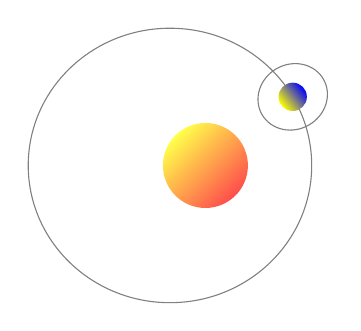
\begin{tikzpicture}[scale=1.8]
        \def\rS{0.3}                                % Sun radius

        \def\Earthangle{30}                         % angle wrt to horizontal        
        \def\rE{0.1}                                % Earth radius
                                                    % Major radius of Earth's elliptical orbit = 1
        \def\eE{0.25}                               % Excentricity of Earth's elliptical orbit       
        \pgfmathsetmacro\bE{sqrt(1-\eE*\eE)}        % Minor radius of Earth's elliptical orbit

        \def\Moonangle{-45}                         % angle wrt to horizontal           
        \pgfmathsetmacro\rM{.7*\rE}                 % Moon radius
        \pgfmathsetmacro\aM{2.5*\rE}                % Major radius of the Moon's elliptical orbit
        \def\eM{0.4}                                % Excentricity of Earth's elliptical orbit
        \pgfmathsetmacro\bM{\aM*sqrt(1-\eM*\eM)}    % Minor radius of the Moon's elliptical orbit 
        \def\offsetM{30}                            % angle offset between the major axes of Earth's and the Moon's orbits



        % This function computes the direction in which light hits the Earth.
        \pgfmathdeclarefunction{f}{1}{%
            \pgfmathparse{
                ((-\eE+cos(#1))<0) * ( 180 + atan( \bE*sin(#1)/(-\eE+cos(#1)) ) ) 
                +
                ((-\eE+cos(#1))>=0) * ( atan( \bE*sin(#1)/(-\eE+cos(#1)) ) ) 
            }
        }

        % This function computes the distance between Earth and the Sun,
        % which is used to calculate the varying radiation intensity on Earth.
        \pgfmathdeclarefunction{d}{1}{%
            \pgfmathparse{ sqrt((-\eE+cos(#1))*(-\eE+cos(#1))+\bE*sin(#1)*\bE*sin(#1)) }
        }

        % Draw the elliptical path of the Earth.
        \draw[thin,color=gray] (0,0) ellipse (1 and \bE);

        % Draw the Sun at the right-hand-side focus
        \shade[
            top color=yellow!70,
            bottom color=red!70,
            shading angle={45},
            ] ({sqrt(1-\bE*\bE)},0) circle (\rS);
         %\draw ({sqrt(1-\b*\b)},-\rS) node[below] {Sun};


        % Draw the Earth at \Earthangle
        \pgfmathsetmacro{\radiation}{100*(1-\eE)/(d(\Earthangle)*d(\Earthangle))}
        \colorlet{Earthlight}{yellow!\radiation!blue}
        \shade[%
            top color=Earthlight,%
            bottom color=blue,%
            shading angle={90+f(\Earthangle)},%
        ] ({cos(\Earthangle)},{\bE*sin(\Earthangle)}) circle (\rE);
        %\draw ({cos(\Earthangle)},{\bE*sin(\Earthangle)-\rE}) node[below] {Earth};  

        % Draw the Moon's (circular) orbit and the Moon at \Moonangle
        \draw[thin,color=gray,rotate around={{\offsetM}:({cos(\Earthangle)},{\bE*sin(\Earthangle)})}]
            ({cos(\Earthangle)},{\bE*sin(\Earthangle)}) ellipse ({\aM} and {\bM});
        %\shade[
        %    top color=black!70,
        %    bottom color=black!30,
        %    shading angle={45},
        %]   ({cos(\Earthangle)+\aM*cos(\Moonangle)*cos(\offsetM)-\bM*sin(\Moonangle)*sin(\offsetM)},%
        %    {\bE*sin(\Earthangle)+\aM*cos(\Moonangle)*sin(\offsetM)+\bM*sin(\Moonangle)*cos(\offsetM)}) circle (\rM);   
    \end{tikzpicture}
    \caption{Earth revolution around the sun}
    \label{fig:earth_revolution}
\end{figure}

The wind direction recorded as cardinals directions are also translated in a format expressing the cyclic relation, \texttt{swd} and \texttt{cwd}, respectively the sine and cosine of the angle of the cardinal direction on a wind rose (see Figure \ref{fig:wind_rose}). 

\begin{figure}[H]
    \centering
    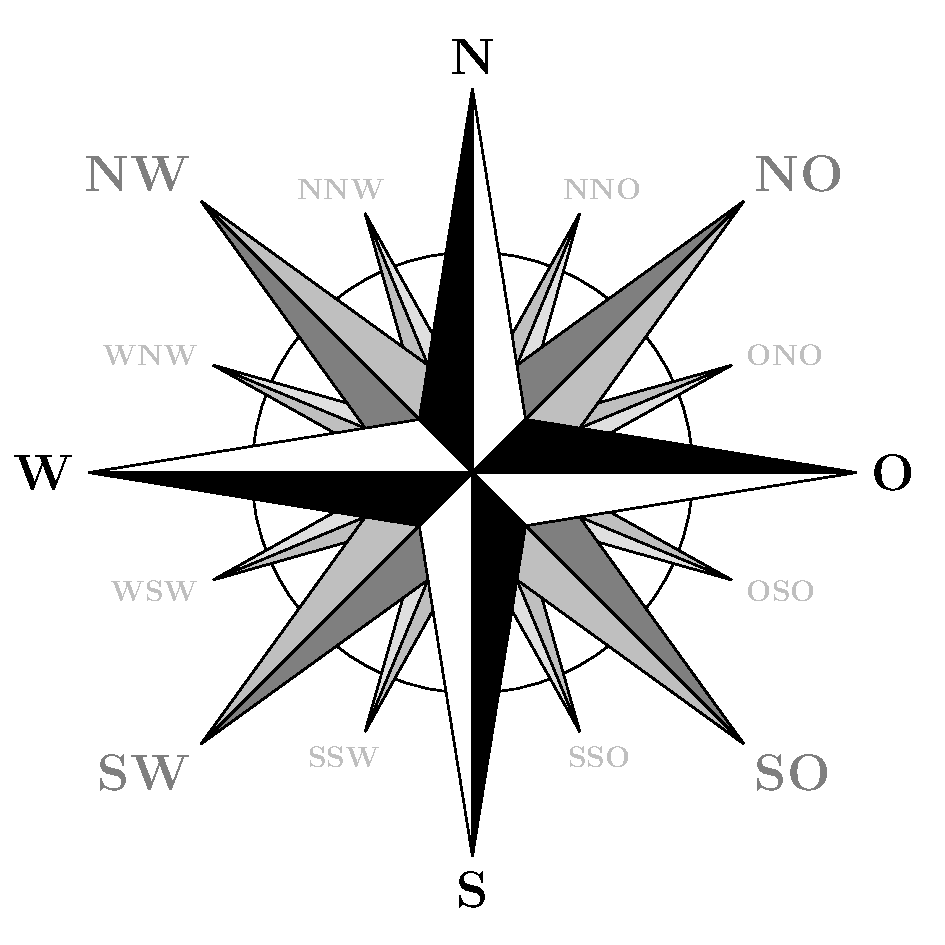
\includegraphics[scale=0.3]{img/compass.pdf}
    \caption{Wind rose}
    \label{fig:wind_rose}
\end{figure}

The complete set of inputs is thus composed of 17 features.
The set of inputs is then normalized using a standard normalization method. 

\section{Features selection}
\label{Features_selection}

Features selection is a technique to drop some less useful inputs. The intrinsic principle aims to maximize the relevance (relation between input and output) and minimize the redundancy (relation between input and input).

It is important to consider the newly created features (cos/sin) in the previous paragraph as a pair of inputs resulting from one unique feature, it is thus not advised to remove one of them  (the sine or cosine) even if they present a high dependency.

\subsection{Correlation}

Figure~\ref{fig:corr} presents the correlation between the inputs and the output (absolute value). Since the correlation only detects linear relations between variables, a zero correlation between an input and the output is not sufficient to drop this input.

\begin{figure}[H]
    \centering
    % This file was created by tikzplotlib v0.8.7.
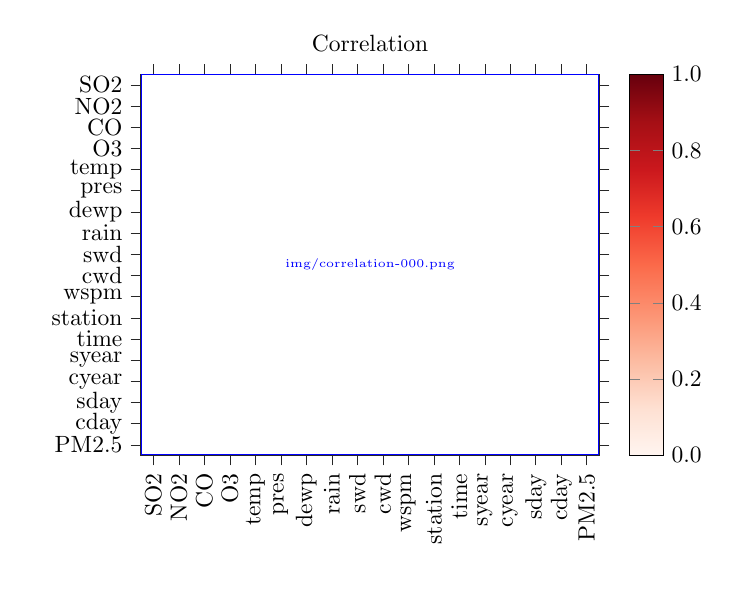
\begin{tikzpicture}[scale=0.85]

\begin{axis}[
axis line style={white!15.0!black},
colorbar,
colorbar style={ytick={0,0.2,0.4,0.6,0.8,1},yticklabels={0.0,0.2,0.4,0.6,0.8,1.0},ylabel={}},
colormap={mymap}{[1pt]
  rgb(0pt)=(1,0.96078431372549,0.941176470588235);
  rgb(1pt)=(0.996078431372549,0.87843137254902,0.823529411764706);
  rgb(2pt)=(0.988235294117647,0.733333333333333,0.631372549019608);
  rgb(3pt)=(0.988235294117647,0.572549019607843,0.447058823529412);
  rgb(4pt)=(0.984313725490196,0.415686274509804,0.290196078431373);
  rgb(5pt)=(0.937254901960784,0.231372549019608,0.172549019607843);
  rgb(6pt)=(0.796078431372549,0.0941176470588235,0.113725490196078);
  rgb(7pt)=(0.647058823529412,0.0588235294117647,0.0823529411764706);
  rgb(8pt)=(0.403921568627451,0,0.0509803921568627)
},
point meta max=1,
point meta min=0,
tick align=outside,
title={Correlation},
x grid style={white!80.0!black},
xmin=0, xmax=18,
xtick style={color=white!15.0!black},
xtick={0.5,1.5,2.5,3.5,4.5,5.5,6.5,7.5,8.5,9.5,10.5,11.5,12.5,13.5,14.5,15.5,16.5,17.5},
xticklabel style = {rotate=90.0},
xticklabels={SO2,NO2,CO,O3,temp,pres,dewp,rain,swd,cwd,wspm,station,time,syear,cyear,sday,cday,PM2.5},
y dir=reverse,
y grid style={white!80.0!black},
ymin=0, ymax=18,
ytick style={color=white!15.0!black},
ytick={0.5,1.5,2.5,3.5,4.5,5.5,6.5,7.5,8.5,9.5,10.5,11.5,12.5,13.5,14.5,15.5,16.5,17.5},
yticklabels={SO2,NO2,CO,O3,temp,pres,dewp,rain,swd,cwd,wspm,station,time,syear,cyear,sday,cday,PM2.5}
]
\addplot graphics [includegraphics cmd=\pgfimage,xmin=0, xmax=18, ymin=18, ymax=0] {img/correlation-000.png};
\end{axis}

\end{tikzpicture}

    \caption{Correlation matrix between the inputs and the output}
    \label{fig:corr}
\end{figure}

\subsection{Mutual information}

Figure~\ref{fig:MI} shows the mutual information between the inputs and the output (absolute value). This method is able to detect any dependency between variables and is thus particularly purposeful to select the right features.

\begin{figure}[H]
    \centering
    % This file was created by tikzplotlib v0.8.7.
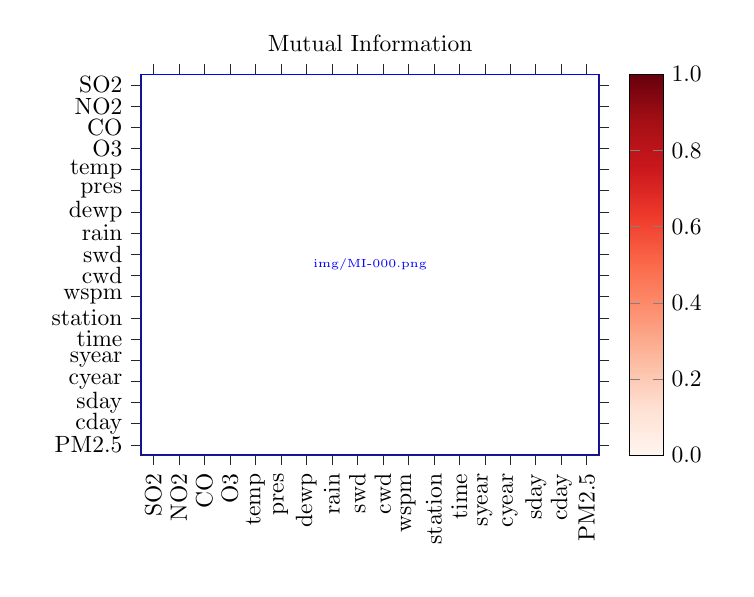
\begin{tikzpicture}[scale=0.85]

\begin{axis}[
axis line style={white!15.0!black},
colorbar,
colorbar style={ytick={0,0.2,0.4,0.6,0.8,1},yticklabels={0.0,0.2,0.4,0.6,0.8,1.0},ylabel={}},
colormap={mymap}{[1pt]
  rgb(0pt)=(1,0.96078431372549,0.941176470588235);
  rgb(1pt)=(0.996078431372549,0.87843137254902,0.823529411764706);
  rgb(2pt)=(0.988235294117647,0.733333333333333,0.631372549019608);
  rgb(3pt)=(0.988235294117647,0.572549019607843,0.447058823529412);
  rgb(4pt)=(0.984313725490196,0.415686274509804,0.290196078431373);
  rgb(5pt)=(0.937254901960784,0.231372549019608,0.172549019607843);
  rgb(6pt)=(0.796078431372549,0.0941176470588235,0.113725490196078);
  rgb(7pt)=(0.647058823529412,0.0588235294117647,0.0823529411764706);
  rgb(8pt)=(0.403921568627451,0,0.0509803921568627)
},
point meta max=1,
point meta min=0,
tick align=outside,
title={Mutual Information},
x grid style={white!80.0!black},
xmin=0, xmax=18,
xtick style={color=white!15.0!black},
xtick={0.5,1.5,2.5,3.5,4.5,5.5,6.5,7.5,8.5,9.5,10.5,11.5,12.5,13.5,14.5,15.5,16.5,17.5},
xticklabel style = {rotate=90.0},
xticklabels={SO2,NO2,CO,O3,temp,pres,dewp,rain,swd,cwd,wspm,station,time,syear,cyear,sday,cday,PM2.5},
y dir=reverse,
y grid style={white!80.0!black},
ymin=0, ymax=18,
ytick style={color=white!15.0!black},
ytick={0.5,1.5,2.5,3.5,4.5,5.5,6.5,7.5,8.5,9.5,10.5,11.5,12.5,13.5,14.5,15.5,16.5,17.5},
yticklabels={SO2,NO2,CO,O3,temp,pres,dewp,rain,swd,cwd,wspm,station,time,syear,cyear,sday,cday,PM2.5}
]
\addplot graphics [includegraphics cmd=\pgfimage,xmin=0, xmax=18, ymin=18, ymax=0] {img/MI-000.png};
\end{axis}

\end{tikzpicture}

    \caption{Mutual Information matrix between the inputs and the output}
    \label{fig:MI}
\end{figure}

\subsection{Redundancy and relevance}

Based on the correlation and MI obtained above, one can drop the features in Table~\ref{tab:relevance} because they have few relevance with the output.

\begin{table}[H]
\setlength\abovecaptionskip{-2\baselineskip}
\centering
\begin{tabular}{cc}
\hline
Feature &  MI with output  \\ \hline
\texttt{station} &  0.074  \\
\texttt{rain}    &  0.079  \\
\texttt{swd}  &  0.098   \\
\texttt{cwd}  &  0.1   \\
\texttt{sday}  &  0.11   \\
\texttt{cday}  &  0.11   \\
\texttt{wspm}  &  0.18   \\ \hline
\end{tabular}
\vspace*{3mm}
\caption{Non relevant features}
\label{tab:relevance}
\end{table}

Additionally, it is possible to remove the temperature (see Table~\ref{tab:temp}), the pressure (see Table~\ref{tab:pres}) and the time (see Table~\ref{tab:time}) since they are redundant with other inputs.

\begin{table}[H]
\setlength\abovecaptionskip{-2\baselineskip}
\centering
\begin{tabular}{ccc}
\hline
Feature &  MI & Correlation \\ \hline
 \texttt{dewp}  & 0.57  & 0.81  \\
 \texttt{cyear}  & 0.79  &  0.9 \\ \hline
\end{tabular}
\vspace*{3mm}
\caption{Relations between some features and a redundant feature: Temperature}
\label{tab:temp}
\end{table}

\begin{table}[H]
\setlength\abovecaptionskip{-2\baselineskip}
\centering
\begin{tabular}{ccc}
\hline
Feature &  MI & Correlation \\ \hline
 \texttt{dewp}  & 0.54  & 0.74  \\
 \texttt{cyear}  & 0.79  &  0.82 \\ \hline
\end{tabular}
\vspace*{3mm}
\caption{Relations between some features and a redundant feature: Pressure}
\label{tab:pres}
\end{table}

It is worth noting that the dependencies between the time and the other features is non linear, such that a small correlation is computed.

\begin{table}[H]
\setlength\abovecaptionskip{-2\baselineskip}
\centering
\begin{tabular}{ccc}
\hline
Feature &  MI & Correlation \\ \hline
  \texttt{syear}  & 0.99  & 0.1  \\
 \texttt{cyear}  & 0.99  &  0.17 \\ \hline
\end{tabular}
\vspace*{3mm}
\caption{Relations between some features and a redundant feature: Time}
\label{tab:time}
\end{table}

Finally, the set resulting of features selection contains 7 features.

\section{Features extraction}
\label{Features_extraction}


Features extraction consists to transform the input into other features such that this new smaller set of features almost fully describes the content of the inputs.

\subsection{Principal Component Analysis}

The Principal Component Analysis method uses an orthogonal transformation to convert a set of inputs into a set of linearly uncorrelated variables called principal components~\cite{pca}.

Figure~\ref{fig:error_PCA} depicts the error for several numbers of principal components, ranging from 1 to 17 (the full number of features). One can conclude that the most important correlation of the data are combined in 3 principal components, lowering the error to \SI{55.5}{\micro g/m^3}. Adding more components does not lead to better results considering that having only 3 input features brings very efficient computations.

However, it is important to note that this method is linear and thus drops important variables if they are non-linearly dependent. This problem depends upon the linear characteristics of the input features. It is consequent for the data analysed here and hence leads to bad results as discussed thereafter.

\begin{figure}[H]
    \centering
    % This file was created by tikzplotlib v0.8.7.
\begin{tikzpicture}[scale=0.9]

\definecolor{color0}{rgb}{0.12156862745098,0.466666666666667,0.705882352941177}

\begin{axis}[
tick align=outside,
tick pos=left,
x grid style={white!69.01960784313725!black},
xlabel={Number of principal components},
xmin=0.19260752688172, xmax=17.8073924731183,
xtick style={color=black},
y grid style={white!69.01960784313725!black},
ylabel={Error [\si{\micro g/m^3}]},
ymin=42.6851630004782, ymax=79.2977079275468,
ytick style={color=black}
]
\addplot [only marks, mark size = 1pt, draw=color0, fill=color0, colormap/viridis]
table{%
x                      y
1 77.6243034002912
2 62.0313757739748
3 55.4915777209778
4 54.7920125917892
5 54.6147880445389
6 54.5912487235166
7 54.046716471317
8 53.8835233713786
9 51.336172028788
10 49.4295859147594
11 48.9092447801225
12 48.537668410929
13 46.4718747248773
14 46.5325938771456
15 46.4760167500513
16 45.0439237982747
17 44.3585675277337
};
\end{axis}

\end{tikzpicture}

    \caption{Bootstrap 632 error for different numbers of principal components}
    \label{fig:error_PCA}
\end{figure}

\section{Error estimation}
\label{Error_estimation}

The errors of the following models are estimated thanks to the Bootstrap 632 method gently provided in the MLxtend package \cite{raschkas_2018_mlxtend}. This highly efficient method is characterized by a low bias and a low variance, which makes it particularly purposeful for model validation (compared to the simpler K-fold validation for instance). If not mentioned in the following sections, the number of splits in the Bootstrap method is set to 10 due to the limited available computation power in classical computers. This small number only influences the randomness of the bootstrap error but not the mean value (most important part).

Figure~\ref{fig:error_analysis_bootstrap} shows the error distribution of the linear regression model with the selected features, for 1 and 10 splits. The error is very narrow for 10 splits ($\sigma = \SI{0.255}{\micro g/m^3}$) compared to 1 split ($\sigma = \SI{0.762}{\micro g/m^3}$), computing the error with 10 splits is thus cogent.

\begin{figure}[H]
    \centering
    % This file was created by tikzplotlib v0.8.7.
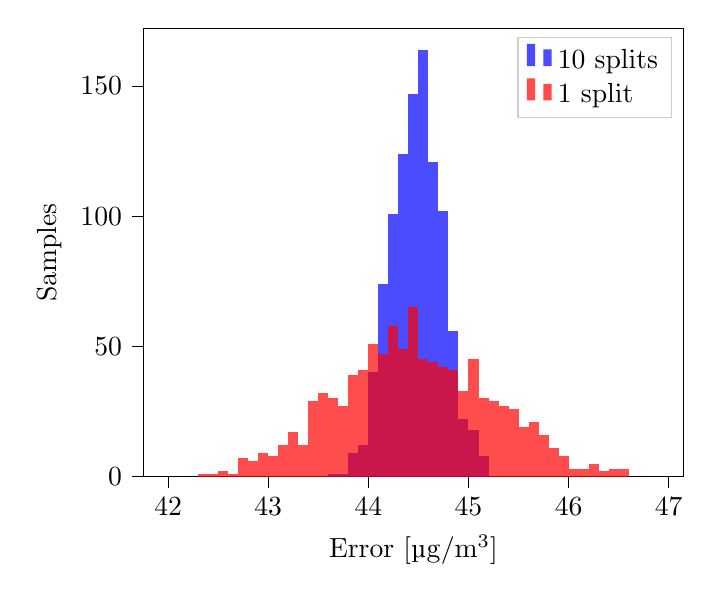
\begin{tikzpicture}

\begin{axis}[
legend cell align={left},
legend style={fill opacity=0.8, draw opacity=1, text opacity=1, draw=white!80.0!black},
tick align=outside,
tick pos=left,
x grid style={white!69.01960784313725!black},
xlabel={Error [\si{\micro g/m^3}]},
xmin=41.755, xmax=47.1450000000001,
xtick style={color=black},
y grid style={white!69.01960784313725!black},
ylabel={Samples},
ymin=0, ymax=172.2,
ytick style={color=black}
]
\draw[fill=blue,draw opacity=0,fill opacity=0.7] (axis cs:42,0) rectangle (axis cs:42.1,0);
\addlegendimage{ybar,ybar legend,fill=blue,draw opacity=0,fill opacity=0.7};
\addlegendentry{10 splits}

\draw[fill=blue,draw opacity=0,fill opacity=0.7] (axis cs:42.1,0) rectangle (axis cs:42.2,0);
\draw[fill=blue,draw opacity=0,fill opacity=0.7] (axis cs:42.2,0) rectangle (axis cs:42.3,0);
\draw[fill=blue,draw opacity=0,fill opacity=0.7] (axis cs:42.3,0) rectangle (axis cs:42.4,0);
\draw[fill=blue,draw opacity=0,fill opacity=0.7] (axis cs:42.4,0) rectangle (axis cs:42.5,0);
\draw[fill=blue,draw opacity=0,fill opacity=0.7] (axis cs:42.5,0) rectangle (axis cs:42.6,0);
\draw[fill=blue,draw opacity=0,fill opacity=0.7] (axis cs:42.6,0) rectangle (axis cs:42.7,0);
\draw[fill=blue,draw opacity=0,fill opacity=0.7] (axis cs:42.7,0) rectangle (axis cs:42.8,0);
\draw[fill=blue,draw opacity=0,fill opacity=0.7] (axis cs:42.8,0) rectangle (axis cs:42.9,0);
\draw[fill=blue,draw opacity=0,fill opacity=0.7] (axis cs:42.9,0) rectangle (axis cs:43,0);
\draw[fill=blue,draw opacity=0,fill opacity=0.7] (axis cs:43,0) rectangle (axis cs:43.1,0);
\draw[fill=blue,draw opacity=0,fill opacity=0.7] (axis cs:43.1,0) rectangle (axis cs:43.2,0);
\draw[fill=blue,draw opacity=0,fill opacity=0.7] (axis cs:43.2,0) rectangle (axis cs:43.3,0);
\draw[fill=blue,draw opacity=0,fill opacity=0.7] (axis cs:43.3,0) rectangle (axis cs:43.4,0);
\draw[fill=blue,draw opacity=0,fill opacity=0.7] (axis cs:43.4,0) rectangle (axis cs:43.5,0);
\draw[fill=blue,draw opacity=0,fill opacity=0.7] (axis cs:43.5,0) rectangle (axis cs:43.6,0);
\draw[fill=blue,draw opacity=0,fill opacity=0.7] (axis cs:43.6,0) rectangle (axis cs:43.7,1);
\draw[fill=blue,draw opacity=0,fill opacity=0.7] (axis cs:43.7,0) rectangle (axis cs:43.8,1);
\draw[fill=blue,draw opacity=0,fill opacity=0.7] (axis cs:43.8,0) rectangle (axis cs:43.9,9);
\draw[fill=blue,draw opacity=0,fill opacity=0.7] (axis cs:43.9,0) rectangle (axis cs:44,12);
\draw[fill=blue,draw opacity=0,fill opacity=0.7] (axis cs:44,0) rectangle (axis cs:44.1,40);
\draw[fill=blue,draw opacity=0,fill opacity=0.7] (axis cs:44.1,0) rectangle (axis cs:44.2,74);
\draw[fill=blue,draw opacity=0,fill opacity=0.7] (axis cs:44.2,0) rectangle (axis cs:44.3,101);
\draw[fill=blue,draw opacity=0,fill opacity=0.7] (axis cs:44.3,0) rectangle (axis cs:44.4,124);
\draw[fill=blue,draw opacity=0,fill opacity=0.7] (axis cs:44.4,0) rectangle (axis cs:44.5,147);
\draw[fill=blue,draw opacity=0,fill opacity=0.7] (axis cs:44.5,0) rectangle (axis cs:44.6,164);
\draw[fill=blue,draw opacity=0,fill opacity=0.7] (axis cs:44.6,0) rectangle (axis cs:44.7,121);
\draw[fill=blue,draw opacity=0,fill opacity=0.7] (axis cs:44.7,0) rectangle (axis cs:44.8,102);
\draw[fill=blue,draw opacity=0,fill opacity=0.7] (axis cs:44.8,0) rectangle (axis cs:44.9,56);
\draw[fill=blue,draw opacity=0,fill opacity=0.7] (axis cs:44.9,0) rectangle (axis cs:45,22);
\draw[fill=blue,draw opacity=0,fill opacity=0.7] (axis cs:45,0) rectangle (axis cs:45.1,18);
\draw[fill=blue,draw opacity=0,fill opacity=0.7] (axis cs:45.1000000000001,0) rectangle (axis cs:45.2000000000001,8);
\draw[fill=blue,draw opacity=0,fill opacity=0.7] (axis cs:45.2,0) rectangle (axis cs:45.3,0);
\draw[fill=blue,draw opacity=0,fill opacity=0.7] (axis cs:45.3000000000001,0) rectangle (axis cs:45.4000000000001,0);
\draw[fill=blue,draw opacity=0,fill opacity=0.7] (axis cs:45.4,0) rectangle (axis cs:45.5,0);
\draw[fill=blue,draw opacity=0,fill opacity=0.7] (axis cs:45.5000000000001,0) rectangle (axis cs:45.6000000000001,0);
\draw[fill=blue,draw opacity=0,fill opacity=0.7] (axis cs:45.6000000000001,0) rectangle (axis cs:45.7000000000001,0);
\draw[fill=blue,draw opacity=0,fill opacity=0.7] (axis cs:45.7000000000001,0) rectangle (axis cs:45.8000000000001,0);
\draw[fill=blue,draw opacity=0,fill opacity=0.7] (axis cs:45.8000000000001,0) rectangle (axis cs:45.9000000000001,0);
\draw[fill=blue,draw opacity=0,fill opacity=0.7] (axis cs:45.9000000000001,0) rectangle (axis cs:46.0000000000001,0);
\draw[fill=blue,draw opacity=0,fill opacity=0.7] (axis cs:46.0000000000001,0) rectangle (axis cs:46.1000000000001,0);
\draw[fill=blue,draw opacity=0,fill opacity=0.7] (axis cs:46.1000000000001,0) rectangle (axis cs:46.2000000000001,0);
\draw[fill=blue,draw opacity=0,fill opacity=0.7] (axis cs:46.2000000000001,0) rectangle (axis cs:46.3000000000001,0);
\draw[fill=blue,draw opacity=0,fill opacity=0.7] (axis cs:46.3000000000001,0) rectangle (axis cs:46.4000000000001,0);
\draw[fill=blue,draw opacity=0,fill opacity=0.7] (axis cs:46.4000000000001,0) rectangle (axis cs:46.5000000000001,0);
\draw[fill=blue,draw opacity=0,fill opacity=0.7] (axis cs:46.5000000000001,0) rectangle (axis cs:46.6000000000001,0);
\draw[fill=blue,draw opacity=0,fill opacity=0.7] (axis cs:46.6000000000001,0) rectangle (axis cs:46.7000000000001,0);
\draw[fill=blue,draw opacity=0,fill opacity=0.7] (axis cs:46.7000000000001,0) rectangle (axis cs:46.8000000000001,0);
\draw[fill=blue,draw opacity=0,fill opacity=0.7] (axis cs:46.8000000000001,0) rectangle (axis cs:46.9000000000001,0);
\draw[fill=red,draw opacity=0,fill opacity=0.7] (axis cs:42,0) rectangle (axis cs:42.1,0);
\addlegendimage{ybar,ybar legend,fill=red,draw opacity=0,fill opacity=0.7};
\addlegendentry{1 split}

\draw[fill=red,draw opacity=0,fill opacity=0.7] (axis cs:42.1,0) rectangle (axis cs:42.2,0);
\draw[fill=red,draw opacity=0,fill opacity=0.7] (axis cs:42.2,0) rectangle (axis cs:42.3,0);
\draw[fill=red,draw opacity=0,fill opacity=0.7] (axis cs:42.3,0) rectangle (axis cs:42.4,1);
\draw[fill=red,draw opacity=0,fill opacity=0.7] (axis cs:42.4,0) rectangle (axis cs:42.5,1);
\draw[fill=red,draw opacity=0,fill opacity=0.7] (axis cs:42.5,0) rectangle (axis cs:42.6,2);
\draw[fill=red,draw opacity=0,fill opacity=0.7] (axis cs:42.6,0) rectangle (axis cs:42.7,1);
\draw[fill=red,draw opacity=0,fill opacity=0.7] (axis cs:42.7,0) rectangle (axis cs:42.8,7);
\draw[fill=red,draw opacity=0,fill opacity=0.7] (axis cs:42.8,0) rectangle (axis cs:42.9,6);
\draw[fill=red,draw opacity=0,fill opacity=0.7] (axis cs:42.9,0) rectangle (axis cs:43,9);
\draw[fill=red,draw opacity=0,fill opacity=0.7] (axis cs:43,0) rectangle (axis cs:43.1,8);
\draw[fill=red,draw opacity=0,fill opacity=0.7] (axis cs:43.1,0) rectangle (axis cs:43.2,12);
\draw[fill=red,draw opacity=0,fill opacity=0.7] (axis cs:43.2,0) rectangle (axis cs:43.3,17);
\draw[fill=red,draw opacity=0,fill opacity=0.7] (axis cs:43.3,0) rectangle (axis cs:43.4,12);
\draw[fill=red,draw opacity=0,fill opacity=0.7] (axis cs:43.4,0) rectangle (axis cs:43.5,29);
\draw[fill=red,draw opacity=0,fill opacity=0.7] (axis cs:43.5,0) rectangle (axis cs:43.6,32);
\draw[fill=red,draw opacity=0,fill opacity=0.7] (axis cs:43.6,0) rectangle (axis cs:43.7,30);
\draw[fill=red,draw opacity=0,fill opacity=0.7] (axis cs:43.7,0) rectangle (axis cs:43.8,27);
\draw[fill=red,draw opacity=0,fill opacity=0.7] (axis cs:43.8,0) rectangle (axis cs:43.9,39);
\draw[fill=red,draw opacity=0,fill opacity=0.7] (axis cs:43.9,0) rectangle (axis cs:44,41);
\draw[fill=red,draw opacity=0,fill opacity=0.7] (axis cs:44,0) rectangle (axis cs:44.1,51);
\draw[fill=red,draw opacity=0,fill opacity=0.7] (axis cs:44.1,0) rectangle (axis cs:44.2,47);
\draw[fill=red,draw opacity=0,fill opacity=0.7] (axis cs:44.2,0) rectangle (axis cs:44.3,58);
\draw[fill=red,draw opacity=0,fill opacity=0.7] (axis cs:44.3,0) rectangle (axis cs:44.4,49);
\draw[fill=red,draw opacity=0,fill opacity=0.7] (axis cs:44.4,0) rectangle (axis cs:44.5,65);
\draw[fill=red,draw opacity=0,fill opacity=0.7] (axis cs:44.5,0) rectangle (axis cs:44.6,45);
\draw[fill=red,draw opacity=0,fill opacity=0.7] (axis cs:44.6,0) rectangle (axis cs:44.7,44);
\draw[fill=red,draw opacity=0,fill opacity=0.7] (axis cs:44.7,0) rectangle (axis cs:44.8,42);
\draw[fill=red,draw opacity=0,fill opacity=0.7] (axis cs:44.8,0) rectangle (axis cs:44.9,41);
\draw[fill=red,draw opacity=0,fill opacity=0.7] (axis cs:44.9,0) rectangle (axis cs:45,33);
\draw[fill=red,draw opacity=0,fill opacity=0.7] (axis cs:45,0) rectangle (axis cs:45.1,45);
\draw[fill=red,draw opacity=0,fill opacity=0.7] (axis cs:45.1000000000001,0) rectangle (axis cs:45.2000000000001,30);
\draw[fill=red,draw opacity=0,fill opacity=0.7] (axis cs:45.2,0) rectangle (axis cs:45.3,29);
\draw[fill=red,draw opacity=0,fill opacity=0.7] (axis cs:45.3000000000001,0) rectangle (axis cs:45.4000000000001,27);
\draw[fill=red,draw opacity=0,fill opacity=0.7] (axis cs:45.4,0) rectangle (axis cs:45.5,26);
\draw[fill=red,draw opacity=0,fill opacity=0.7] (axis cs:45.5000000000001,0) rectangle (axis cs:45.6000000000001,19);
\draw[fill=red,draw opacity=0,fill opacity=0.7] (axis cs:45.6000000000001,0) rectangle (axis cs:45.7000000000001,21);
\draw[fill=red,draw opacity=0,fill opacity=0.7] (axis cs:45.7000000000001,0) rectangle (axis cs:45.8000000000001,16);
\draw[fill=red,draw opacity=0,fill opacity=0.7] (axis cs:45.8000000000001,0) rectangle (axis cs:45.9000000000001,11);
\draw[fill=red,draw opacity=0,fill opacity=0.7] (axis cs:45.9000000000001,0) rectangle (axis cs:46.0000000000001,8);
\draw[fill=red,draw opacity=0,fill opacity=0.7] (axis cs:46.0000000000001,0) rectangle (axis cs:46.1000000000001,3);
\draw[fill=red,draw opacity=0,fill opacity=0.7] (axis cs:46.1000000000001,0) rectangle (axis cs:46.2000000000001,3);
\draw[fill=red,draw opacity=0,fill opacity=0.7] (axis cs:46.2000000000001,0) rectangle (axis cs:46.3000000000001,5);
\draw[fill=red,draw opacity=0,fill opacity=0.7] (axis cs:46.3000000000001,0) rectangle (axis cs:46.4000000000001,2);
\draw[fill=red,draw opacity=0,fill opacity=0.7] (axis cs:46.4000000000001,0) rectangle (axis cs:46.5000000000001,3);
\draw[fill=red,draw opacity=0,fill opacity=0.7] (axis cs:46.5000000000001,0) rectangle (axis cs:46.6000000000001,3);
\draw[fill=red,draw opacity=0,fill opacity=0.7] (axis cs:46.6000000000001,0) rectangle (axis cs:46.7000000000001,0);
\draw[fill=red,draw opacity=0,fill opacity=0.7] (axis cs:46.7000000000001,0) rectangle (axis cs:46.8000000000001,0);
\draw[fill=red,draw opacity=0,fill opacity=0.7] (axis cs:46.8000000000001,0) rectangle (axis cs:46.9000000000001,0);
\end{axis}

\end{tikzpicture}

    \caption{Bootstrap 632 error distribution for different numbers of splits}
    \label{fig:error_analysis_bootstrap}
\end{figure}

\section{Models implementations}
\label{Models_implementations}


Seven models have been trained and compared in order to bring the most powerful one for the estimation of the secret dataset. These models are tested with the bootstrap 632 error on the three previously detailed input sets: the full features, the selected features and the PCA features.

Let the dataset be $D = { (x_1 , y_1 ),(x_2 , y_2 ),\ldots,(x_N , y_N ) }$ where  $x_i$ is the input value and $y_i$ is the target value, the goal of a regression model is to estimate the function $y = f(x)$.

\subsection{Linear regression}
 
The linear regression estimates the function $y = f(x)$ by $\hat{f}(x) = w^Tx$. The weight vector $w$ is computed by minimizing the mean squared error on the training data: $$\displaystyle \min_{\mathbf{w}} ||\mathbf{y}_{\text{train}} - \mathbf{w}^T\mathbf{X}_{\text{train}}||_2^2.$$

The error for the three implemented sets is given in Table~\ref{tab:linreg}. One can see that the 7 selected features give almost the same error as for the full input set, which validates the features selection (at least for linear models). However, the PCA method, although very fast, is not convincing because it has few features.

\begin{table}[H]
\setlength\abovecaptionskip{-2\baselineskip}
\centering
\begin{tabular}{cc}
\hline
 Features &  Error [\si{\micro g/m^3}] \\ \hline
 Full  & 44.35 \\
 Selected  & 44.50 \\
 PCA  & 54.10 \\ \hline
\end{tabular}
\vspace*{3mm}
\caption{Bootstrap 632 error for the Linear regression model}
\label{tab:linreg}
\end{table}

\subsection{Ridge regression}

The ridge regression is similar to the linear regression with a shrinkage penalty on $\mathbf{w}$ ($L_2$ regularization): $$\displaystyle \min_{\mathbf{w}} ||\mathbf{y}_{\text{train}} - \mathbf{w}^T\mathbf{X}_{\text{train}}||_2^2 + \lambda ||\mathbf{w}||_2^2.$$
The parameter $\lambda$ controls the relative impact of the two terms. Increasing $\lambda$ decreases the variance while increasing the bias. 

As shown in Figure~\ref{fig:RR}, the ridge regression performs better with the \textit{selected features} and \textit{full features} than with the \textit{PCA features}. The performance is almost constant for $\lambda \in [10^{-2},10^2]$ and decreases after when the model starts to suffer from underfitting. The best result is achieved with the \textit{full features} and $\lambda = 0.61$, the error is \SI{44.15}{\micro g/m^3}. 

\begin{figure}[H]
    \centering
    % This file was created by tikzplotlib v0.8.7.
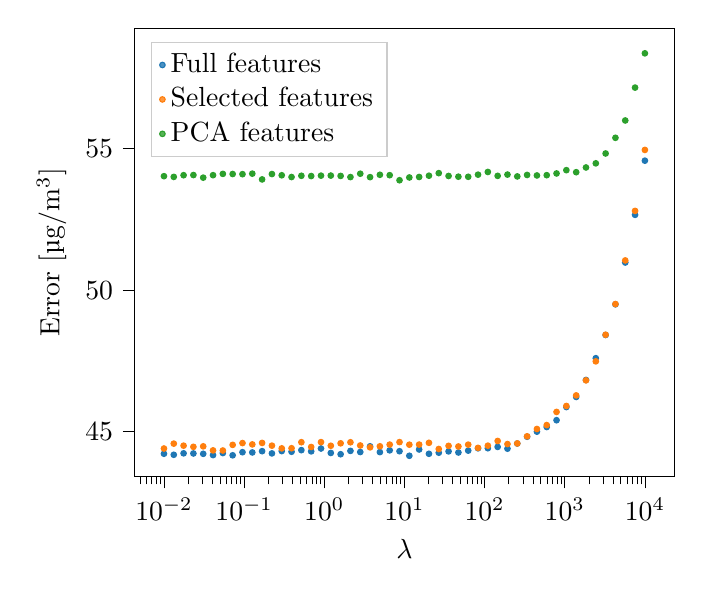
\begin{tikzpicture}

\definecolor{color0}{rgb}{0.12156862745098,0.466666666666667,0.705882352941177}
\definecolor{color1}{rgb}{1,0.498039215686275,0.0549019607843137}
\definecolor{color2}{rgb}{0.172549019607843,0.627450980392157,0.172549019607843}

\begin{axis}[
legend cell align={left},
legend style={fill opacity=0.8, draw opacity=1, text opacity=1, at={(0.03,0.97)}, anchor=north west, draw=white!80.0!black},
log basis x={10},
tick align = outside,
tick pos=left,
x grid style={white!69.01960784313725!black},
xlabel={$\lambda$},
xmin=0.00430189297194492, xmax=23245.5806437206,
xmode=log,
xtick style={color=black},
y grid style={white!69.01960784313725!black},
ylabel={Error [\si{\micro g/m^3}]},
ymin=43.4115392449125, ymax=59.2539921320645,
ytick style={color=black}
]
\addplot [only marks, mark size=1pt, draw=color0, fill=color0, colormap/viridis]
table{%
x                      y
0.01 44.2167889948757
0.0132571136559011 44.1807666923535
0.0175751062485479 44.2320421734545
0.0232995181051537 44.2276324649521
0.0308884359647748 44.2149239431597
0.0409491506238043 44.1697886781025
0.0542867543932386 44.2424837596312
0.0719685673001152 44.1624044079414
0.0954095476349994 44.271640601243
0.12648552168553 44.2627266684372
0.167683293681101 44.3080433032249
0.222299648252619 44.2299750252643
0.294705170255181 44.3111167482614
0.390693993705462 44.2876236605304
0.517947467923121 44.3446307986795
0.6866488450043 44.3013778043881
0.910298177991522 44.4026568192283
1.20679264063933 44.2453240022826
1.59985871960606 44.1996691921372
2.12095088792019 44.3184803061784
2.81176869797423 44.2778221358281
3.72759372031494 44.4799484014015
4.94171336132383 44.2747022437435
6.55128556859551 44.337125647165
8.68511373751352 44.3066244589908
11.5139539932645 44.1454476492753
15.2641796717523 44.3677422866312
20.2358964772516 44.2156921957473
26.8269579527972 44.2540838789006
35.5648030622313 44.3008287914991
47.1486636345739 44.2618717478643
62.5055192527397 44.3276283704093
82.8642772854684 44.4094152433137
109.854114198756 44.4127328650544
145.634847750124 44.4585229580228
193.069772888325 44.396584963084
255.954792269953 44.5790118994576
339.322177189533 44.8192178112522
449.843266896944 44.9973217658132
596.362331659464 45.1614498331597
790.60432109077 45.4020668149435
1048.11313415469 45.8675739709525
1389.49549437314 46.224090352221
1842.06996932672 46.8245167299567
2442.05309454865 47.5942134722938
3237.45754281764 48.4145047650417
4291.93426012878 49.497188077793
5689.86602901829 50.9746173479057
7543.12006335461 52.6596188921184
10000 54.5732738470204
};
\addlegendentry{Full features}
\addplot [only marks, mark size=1pt, draw=color1, fill=color1, colormap/viridis]
table{%
x                      y
0.01 44.4023865046758
0.0132571136559011 44.5745116510722
0.0175751062485479 44.503220131335
0.0232995181051537 44.4614583375721
0.0308884359647748 44.4793096804501
0.0409491506238043 44.335967774784
0.0542867543932386 44.3315469861985
0.0719685673001152 44.5309227854363
0.0954095476349994 44.5944538919496
0.12648552168553 44.5477377996225
0.167683293681101 44.5997738748121
0.222299648252619 44.5033469595212
0.294705170255181 44.4077895541168
0.390693993705462 44.4123754619294
0.517947467923121 44.6251818128717
0.6866488450043 44.4559572087253
0.910298177991522 44.6275522429277
1.20679264063933 44.4993509242715
1.59985871960606 44.5856437655494
2.12095088792019 44.6226744362044
2.81176869797423 44.5099012211242
3.72759372031494 44.4439205988496
4.94171336132383 44.4805328260223
6.55128556859551 44.5403291614502
8.68511373751352 44.6284186392793
11.5139539932645 44.537572149237
15.2641796717523 44.5414021514288
20.2358964772516 44.6034559256958
26.8269579527972 44.3848858157808
35.5648030622313 44.4960945576422
47.1486636345739 44.4740198236704
62.5055192527397 44.5387383027436
82.8642772854684 44.4248756376892
109.854114198756 44.5022286410543
145.634847750124 44.6685993008299
193.069772888325 44.5593091731685
255.954792269953 44.5821884925407
339.322177189533 44.8329350519135
449.843266896944 45.092236985923
596.362331659464 45.2297199764255
790.60432109077 45.6953968597213
1048.11313415469 45.9051233260361
1389.49549437314 46.2787034248005
1842.06996932672 46.8107510431027
2442.05309454865 47.4817471016569
3237.45754281764 48.4222668911318
4291.93426012878 49.5073507971491
5689.86602901829 51.0490532811031
7543.12006335461 52.7990664142071
10000 54.9531670858037
};
\addlegendentry{Selected features}
\addplot [only marks, mark size=1pt, draw=color2, fill=color2, colormap/viridis]
table{%
x                      y
0.01 54.0258137856725
0.0132571136559011 54.0001721088575
0.0175751062485479 54.0598572614595
0.0232995181051537 54.0654838636448
0.0308884359647748 53.9736055125927
0.0409491506238043 54.0611316870404
0.0542867543932386 54.1068673483855
0.0719685673001152 54.1020018823889
0.0954095476349994 54.0968479410916
0.12648552168553 54.1147679000287
0.167683293681101 53.9108510421111
0.222299648252619 54.1010874579653
0.294705170255181 54.0579326365081
0.390693993705462 53.9955229841454
0.517947467923121 54.0394348767276
0.6866488450043 54.0303931622094
0.910298177991522 54.0444173291291
1.20679264063933 54.0468812734024
1.59985871960606 54.0344166590579
2.12095088792019 53.9936001359387
2.81176869797423 54.1128723764391
3.72759372031494 53.9908965750729
4.94171336132383 54.0744959466062
6.55128556859551 54.0602096549696
8.68511373751352 53.8821673989544
11.5139539932645 53.9800179103607
15.2641796717523 53.9971788232181
20.2358964772516 54.0421828130749
26.8269579527972 54.1331707662564
35.5648030622313 54.0331388855388
47.1486636345739 54.0078831752934
62.5055192527397 54.0044554667871
82.8642772854684 54.0793733860045
109.854114198756 54.1744505989464
145.634847750124 54.0367738115669
193.069772888325 54.0820640027802
255.954792269953 54.0171812856796
339.322177189533 54.0690394055027
449.843266896944 54.051368207826
596.362331659464 54.0607958412667
790.60432109077 54.1220502383948
1048.11313415469 54.2384847643161
1389.49549437314 54.1665717872289
1842.06996932672 54.3334290106613
2442.05309454865 54.479824413464
3237.45754281764 54.8281773679687
4291.93426012878 55.3816661534625
5689.86602901829 55.9940118756015
7543.12006335461 57.155985747128
10000 58.367238618901
};
\addlegendentry{PCA features}
\end{axis}

\end{tikzpicture}

    \caption{Bootstrap 632 error for the Ridge regression model}
    \label{fig:RR}
\end{figure}

\subsection{Lasso}

The Lasso regression is similar to the ridge regression with a shrinkage penalty on $\mathbf{w}$ ($L_1$ regularization): $$\displaystyle \min_{\mathbf{w}} ||\mathbf{y}_{\text{train}} - \mathbf{w}^T\mathbf{X}_{\text{train}}||_2^2 + \lambda \sum_{i=1}^N |\mathbf{w_i}|.$$

As shown in Figure~\ref{fig:Lasso}, the lasso regression performances are almost constant until $\lambda = 1$ and start to decrease after because of underfitting. Similarly to the ridge regression the Lasso performs better with the \textit{full} and \textit{selected features}. The best result is achieved with the \textit{full features} and $\lambda = 0.01$, the error is \SI{44.06}{\micro g/m^3}. 

\begin{figure}[H]
    \centering
    % This file was created by tikzplotlib v0.8.7.
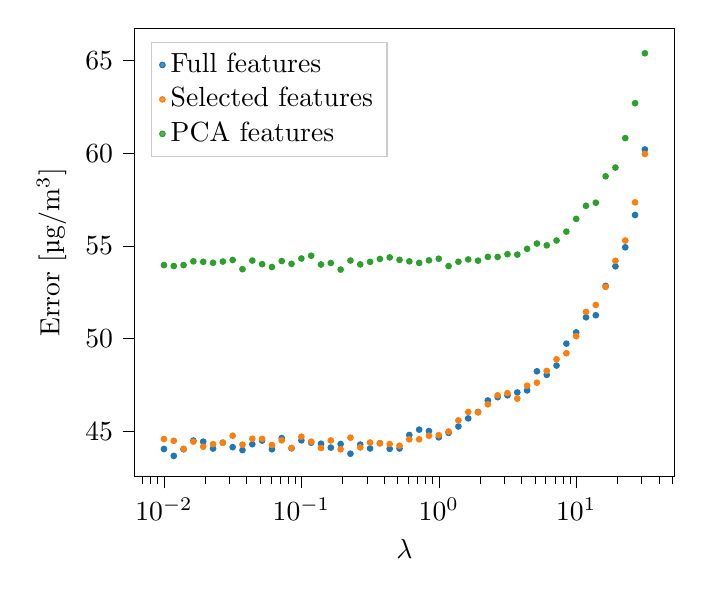
\begin{tikzpicture}

\definecolor{color0}{rgb}{0.12156862745098,0.466666666666667,0.705882352941177}
\definecolor{color1}{rgb}{1,0.498039215686275,0.0549019607843137}
\definecolor{color2}{rgb}{0.172549019607843,0.627450980392157,0.172549019607843}

\begin{axis}[
legend cell align={left},
legend style={fill opacity=0.8, draw opacity=1, text opacity=1, at={(0.03,0.97)}, anchor=north west, draw=white!80.0!black},
log basis x={10},
tick align = outside,
tick pos=left,
x grid style={white!69.01960784313725!black},
xlabel={$\lambda$},
xmin=0.0061136374185611, xmax=51.724978824679,
xmode=log,
xtick style={color=black},
y grid style={white!69.01960784313725!black},
ylabel={Error [\si{\micro g/m^3}]},
ymin=42.5723162048217, ymax=66.7376301720848,
ytick style={color=black}
]
\addplot [only marks, mark size=1pt, draw=color0, fill=color0, colormap/viridis]
table{%
x                      y
0.01 44.0572521836548
0.0117876863479359 43.6845364764623
0.0138949549437314 44.0421580786967
0.0163789370695406 44.5134022921654
0.0193069772888325 44.4546410177915
0.0227584592607479 44.0803835595763
0.0268269579527973 44.4007923162282
0.0316227766016838 44.1575682828234
0.0372759372031494 43.9981903372341
0.0439397056076079 44.3140428075462
0.0517947467923121 44.5105830355541
0.0610540229658533 44.0424793803414
0.0719685673001152 44.644217519812
0.0848342898244072 44.091367192696
0.1 44.5222377181906
0.117876863479359 44.3966908362241
0.138949549437314 44.342568508449
0.163789370695406 44.1321489364452
0.193069772888325 44.3256533426001
0.227584592607479 43.8040050349762
0.268269579527972 44.2959602833513
0.316227766016838 44.0882400290666
0.372759372031494 44.3712508412549
0.439397056076079 44.0656726496125
0.517947467923121 44.0842003888401
0.610540229658533 44.8119527415233
0.719685673001152 45.1020045575328
0.848342898244072 45.0242498155445
1 44.6870191233243
1.17876863479359 44.9259192470893
1.38949549437314 45.2711667543819
1.63789370695406 45.7066918681089
1.93069772888325 46.0520562945631
2.27584592607479 46.6717055170009
2.68269579527972 46.8526010047054
3.16227766016838 46.9499755291371
3.72759372031494 47.1053095596817
4.39397056076079 47.2157993825237
5.17947467923121 48.2456558330529
6.10540229658533 48.0539462671207
7.19685673001151 48.5548886830292
8.48342898244072 49.7367455374351
10 50.3424980904068
11.7876863479359 51.156780805757
13.8949549437314 51.2661223238983
16.3789370695406 52.847877055191
19.3069772888325 53.9022859954272
22.7584592607479 54.9275380246092
26.8269579527972 56.6696414109744
31.6227766016838 60.2025800517163
};
\addlegendentry{Full features}
\addplot [only marks, mark size=1pt, draw=color1, fill=color1, colormap/viridis]
table{%
x                      y
0.01 44.597011622397
0.0117876863479359 44.4994522902063
0.0138949549437314 44.0663331178506
0.0163789370695406 44.4533184060743
0.0193069772888325 44.1822058244549
0.0227584592607479 44.3173606747212
0.0268269579527973 44.3891722662157
0.0316227766016838 44.7768146494824
0.0372759372031494 44.2933737971688
0.0439397056076079 44.6118426122139
0.0517947467923121 44.6014342599006
0.0610540229658533 44.2725387012228
0.0719685673001152 44.5214855098968
0.0848342898244072 44.1125876697293
0.1 44.7192935428211
0.117876863479359 44.4513533262062
0.138949549437314 44.1066157954189
0.163789370695406 44.5174557900556
0.193069772888325 44.0409573455303
0.227584592607479 44.6690155327435
0.268269579527972 44.1437754622129
0.316227766016838 44.4055360426274
0.372759372031494 44.3607636671279
0.439397056076079 44.3248728275886
0.517947467923121 44.2361739858403
0.610540229658533 44.5764915998677
0.719685673001152 44.5793265623022
0.848342898244072 44.7693958287626
1 44.8033144598882
1.17876863479359 44.9997746857396
1.38949549437314 45.597449111305
1.63789370695406 46.0535265385397
1.93069772888325 46.0329168316635
2.27584592607479 46.4640192078204
2.68269579527972 46.9494266205038
3.16227766016838 47.0679667507315
3.72759372031494 46.7709438368159
4.39397056076079 47.4669152116926
5.17947467923121 47.6320153555652
6.10540229658533 48.266089894936
7.19685673001151 48.8928479738715
8.48342898244072 49.2188534279922
10 50.138313537365
11.7876863479359 51.4477588628621
13.8949549437314 51.8218253053721
16.3789370695406 52.7943416312788
19.3069772888325 54.2029175487831
22.7584592607479 55.2930777174122
26.8269579527972 57.3514009045053
31.6227766016838 59.9574954059926
};
\addlegendentry{Selected features}
\addplot [only marks, mark size=1pt, draw=color2, fill=color2, colormap/viridis]
table{%
x                      y
0.01 53.9696272136484
0.0117876863479359 53.9213987429405
0.0138949549437314 53.9704894525133
0.0163789370695406 54.1734407439141
0.0193069772888325 54.1452766420061
0.0227584592607479 54.0918086686184
0.0268269579527973 54.1609738215371
0.0316227766016838 54.2434451583531
0.0372759372031494 53.7495782979567
0.0439397056076079 54.2137062545661
0.0517947467923121 54.0195063487908
0.0610540229658533 53.8661164842485
0.0719685673001152 54.1881517609452
0.0848342898244072 54.0386353324166
0.1 54.3253495068045
0.117876863479359 54.4742880541767
0.138949549437314 54.0020183433581
0.163789370695406 54.0842566914464
0.193069772888325 53.7289476878617
0.227584592607479 54.2151751550016
0.268269579527972 54.007623425378
0.316227766016838 54.1438735851151
0.372759372031494 54.2991343459841
0.439397056076079 54.3837397032873
0.517947467923121 54.2524040085292
0.610540229658533 54.173006692264
0.719685673001152 54.0872737643576
0.848342898244072 54.2263001503516
1 54.3121336000496
1.17876863479359 53.9188327673828
1.38949549437314 54.1503457736495
1.63789370695406 54.2738358664995
1.93069772888325 54.2096691364118
2.27584592607479 54.4099201264293
2.68269579527972 54.4086170676264
3.16227766016838 54.5586261085119
3.72759372031494 54.5356940698227
4.39397056076079 54.8454202552213
5.17947467923121 55.1316547761245
6.10540229658533 55.0346230826969
7.19685673001151 55.2958500902838
8.48342898244072 55.7740278916166
10 56.4601027242987
11.7876863479359 57.165684911882
13.8949549437314 57.3321485079221
16.3789370695406 58.7572492782157
19.3069772888325 59.2276019625299
22.7584592607479 60.8136885282453
26.8269579527972 62.6979093350142
31.6227766016838 65.3881002821541
};
\addlegendentry{PCA features}
\end{axis}

\end{tikzpicture}

    \caption{Bootstrap 632 error for the Lasso model}
    \label{fig:Lasso}
\end{figure}

\begin{figure}[H]
    \centering
    \input{img/Lasso_weights.tex}
    \caption{Weights of the Lasso model ($\lambda = 0.1$)}
    \label{fig:Lasso_weights}
\end{figure}

The weights for $\lambda = 0.1$ are given in Figure~\ref{fig:Lasso_weights}. As found in the features selection, the output is very sensitive to three features, and more or less 7 features completely describe the input space. Some coefficients end up being set to almost zero, making the model easier to interpret.

As both the Ridge regression and Lasso models are better with a small regularization coefficient, they are redundant with the linear regression. This can be explained by the high number of samples used for the training, which are sufficient to prevent overfitting in the linear regression model. These two additional models cannot exploit their advantage of reducing the linear regression overfitting.

\subsection{K-Nearest Neighbour}

Figure~\ref{fig:KNN} presents the error for the KNN model with respect to the number of neighbours $K$ (hyperparameter). For this model, using the full input set should dramatically increase the error since in a high dimensional space, the $K$ nearest neighbours (with the Euclidian norm) are greatly influenced by useless dimensions and thus lead to select wrong neighbours. As expected, the model with features selection outperforms the others, reaching an error of \SI{38.51}{\micro g/m^3} for $K = 4$.


\begin{figure}[H]
    \centering
    % This file was created by tikzplotlib v0.8.7.
\begin{tikzpicture}

\definecolor{color0}{rgb}{0.12156862745098,0.466666666666667,0.705882352941177}
\definecolor{color1}{rgb}{1,0.498039215686275,0.0549019607843137}
\definecolor{color2}{rgb}{0.172549019607843,0.627450980392157,0.172549019607843}

\begin{axis}[
legend cell align={left},
legend style={fill opacity=0.8, draw opacity=1, text opacity=1, at={(0.97,0.03)}, anchor=south east, draw=white!80.0!black},
tick align=outside,
tick pos=left,
x grid style={white!69.01960784313725!black},
xlabel={Neighbours},
xmin=-1.85434704244936, xmax=52.8543470424494,
xtick style={color=black},
y grid style={white!69.01960784313725!black},
ylabel={Error [ug/m\^3]},
ymin=37.7837586360246, ymax=52.8719100227007,
ytick style={color=black}
]
\addplot [only marks, marker=*, draw=color0, fill=color0, colormap/viridis]
table{%
x                      y
1 46.2717177056029
2 44.6427242985358
3 44.1640065447711
4 44.2708127027097
5 44.1193122771592
6 44.167683612613
7 44.2538393324838
8 44.3176295913116
9 44.278516257126
10 44.3825314838463
11 44.5397989481667
12 44.7866831575225
13 44.7066218791601
14 45.0379433828352
15 44.9068996651348
16 45.0446852717636
17 45.2118401612421
18 45.2064408404679
19 45.4356607596669
20 45.5313978975279
21 45.5659089228476
22 45.6555162883844
23 45.5951786992852
24 45.8024140456876
25 45.8867385691758
26 45.9616589938269
27 45.9927985663059
28 45.9864259822899
29 46.2655330512912
30 46.2731469664841
31 46.4783872954807
32 46.3206253088594
33 46.4182156378999
34 46.529168238539
35 46.477353534705
36 46.6887742735855
37 46.6071552022515
38 46.6860717186912
39 46.8654231151779
40 46.941731120255
41 47.0952832472312
42 47.1905251572548
43 47.3012075048838
44 47.1431034772893
45 47.237748101404
46 47.4427345158595
47 47.4695783987426
48 47.534061946931
49 47.4876068044874
50 47.638979776283
};
\addlegendentry{Full features}
\addplot [only marks, marker=*, draw=color1, fill=color1, colormap/viridis]
table{%
x                      y
1 39.7125614350308
2 38.5053808818762
3 38.558684692205
4 38.5177468631443
5 38.5777401657383
6 38.9771575651562
7 38.9291529392842
8 38.8855355874572
9 39.2179799039942
10 39.2327861389491
11 39.1142531473267
12 39.5713032033747
13 39.6716483991726
14 39.5167871043444
15 39.6143329650129
16 39.7493565760095
17 39.678578722464
18 39.7477966585005
19 40.0249017444162
20 40.0369159653303
21 39.9983878411032
22 40.2295340963212
23 40.1776198287666
24 40.2804851775764
25 40.2906006422457
26 40.4566366022387
27 40.4548790341029
28 40.6995023393875
29 40.7151914003398
30 40.7589057132326
31 40.851810303655
32 40.855846115656
33 40.9011119992161
34 40.9980849780594
35 41.1556217680315
36 41.0724669548882
37 41.1487154867687
38 41.3145931272688
39 41.3693127052435
40 41.417046849331
41 41.5113297597832
42 41.6797746887156
43 41.6245705445054
44 41.4724313776891
45 41.8213622768863
46 41.7736673898084
47 41.7937871017152
48 41.9178342792248
49 41.936287222866
50 42.0527653976787
};
\addlegendentry{Selected features}
\addplot [only marks, marker=*, draw=color2, fill=color2, colormap/viridis]
table{%
x                      y
1 52.0932183903306
2 49.8849509928445
3 49.1254291462877
4 48.5844067651702
5 48.9773491184074
6 48.9235761431163
7 48.9584201130001
8 48.943707638385
9 49.0758498964453
10 49.1803905628501
11 49.1417646033178
12 49.2073176212986
13 49.24638054296
14 49.2461265344835
15 49.3245508684918
16 49.4446133299051
17 49.4929809532503
18 49.4983376888973
19 49.4389571918321
20 49.5046861772997
21 49.6179228102202
22 49.6035493832833
23 49.5778639644661
24 49.602885653999
25 49.7208509550203
26 49.757242014041
27 49.788138293316
28 49.8158291451185
29 49.8326013585841
30 49.8354037586306
31 50.0750896552971
32 49.9878695143755
33 50.0157171859563
34 49.9044207652502
35 50.0437564015936
36 50.1233591614317
37 50.0949448847281
38 50.1240367937795
39 50.0383527430695
40 50.3053425601045
41 50.2655463694206
42 50.4297446730343
43 50.2419401890373
44 50.480039493023
45 50.3729887213888
46 50.5184748583874
47 50.3460992647861
48 50.4942276021418
49 50.446578399569
50 50.5038727972999
};
\addlegendentry{PCA features}
\end{axis}

\end{tikzpicture}

    \caption{Bootstrap 632 error for the KNN model}
    \label{fig:KNN}
\end{figure}


\subsection{Regression tree}

A regression tree partitions the input space in smaller regions recursively until reaching a leaf where a simple model is fitted to. Each node represents a binary questions about one or several feature(s) that will divide the space in two.  For a classic regression tree, the model at each leaf is a constant estimate: the average of the target value of the training data that belongs to this leaf. The binary questions on the nodes are chosen such that the information gain is maximized. Mechanisms such as pruning are necessary to avoid overfitting. 


As shown in Figure~\ref{fig:tree}, the performance obtained by the \textit{full} and \textit{selected features} are very close and outperform the ones obtained with the \textit{PCA features}. The performances increase as the maximal depth of the tree increases until reaching a maximum at 7 for the \textit{PCA features}, then it starts to overfit since there are too few features in PCA. The error obtained with the \textit{full} and \textit{selected features} stops decreasing and starts to level out at a depth of around 10. It has to be noted than the trees do not grow further than a depth of 33, explaining the absence of overfitting as the allowed maximal depth continues to increase. The best result is achieved with the \textit{selected features} and a depth of 11, the error is \SI{40.23}{\micro g/m^3}.

\begin{figure}[H]
    \centering
    % This file was created by tikzplotlib v0.8.7.
\begin{tikzpicture}

\definecolor{color0}{rgb}{0.12156862745098,0.466666666666667,0.705882352941177}
\definecolor{color1}{rgb}{1,0.498039215686275,0.0549019607843137}
\definecolor{color2}{rgb}{0.172549019607843,0.627450980392157,0.172549019607843}

\begin{axis}[
legend cell align={left},
legend style={fill opacity=0.8, draw opacity=1, text opacity=1, draw=white!80.0!black},
tick align=outside,
tick pos=both,
x grid style={white!69.01960784313725!black},
xlabel={Max depth},
xmin=-0.160068417197653, xmax=21.1600684171976,
xtick style={color=black},
y grid style={white!69.01960784313725!black},
ylabel={Error [ug/m\^3]},
ymin=38.4382015672962, ymax=73.4236831101486,
ytick style={color=black}
]
\addplot [only marks, marker=*, draw=color0, fill=color0, colormap/viridis]
table{%
x                      y
1 61.4841658097659
2 52.7019214816992
3 49.9388295707787
4 46.6516565850894
5 45.8717628663284
6 44.7885526107626
7 42.5989908236828
8 41.996055370633
9 42.2856496860627
10 41.8497002619999
11 41.7897787653355
12 41.8489404765008
13 42.1243864224217
14 42.4196491832485
15 41.9900012455314
16 41.8795976247328
17 42.3837490939013
18 41.3360172445
19 41.4403947581124
20 42.6068490151299
};
\addlegendentry{Full features}
\addplot [only marks, marker=*, draw=color1, fill=color1, colormap/viridis]
table{%
x                      y
1 61.8351734060708
2 52.2011402694587
3 49.6263834467848
4 47.2319307498906
5 45.2559705658309
6 43.8286416436655
7 42.7909515708027
8 41.4436789803852
9 40.8066911303669
10 40.5357220708065
11 40.9635748147866
12 40.4144810075879
13 40.3346499091113
14 40.7630772527228
15 41.2270566362183
16 41.5790953715711
17 41.391772183205
18 41.2202883697978
19 41.8194817482347
20 42.3665372158653
};
\addlegendentry{Selected features}
\addplot [only marks, marker=*, draw=color2, fill=color2, colormap/viridis]
table{%
x                      y
1 71.4978349694691
2 62.3751401625014
3 58.2614451290866
4 55.410047642098
5 53.6686340559232
6 52.6235618786388
7 51.9263516991862
8 52.72284530217
9 52.4548859103453
10 53.4464615428617
11 53.2439227037874
12 54.1200211370392
13 54.5105153168165
14 54.4933318668924
15 53.7069831521228
16 54.8073346114244
17 54.7489533478021
18 55.0427012271413
19 55.8486074563625
20 54.9090061944327
};
\addlegendentry{PCA features}
\end{axis}

\end{tikzpicture}

    \caption{Bootstrap 632 error for the regression tree model}
    \label{fig:tree}
\end{figure}


\subsection{Bootstrap aggregating trees}

The core idea of an ensemble method is to train weak regressors (or classifiers) and combine them to construct a regressor (or classifier) more powerful than any of the individual ones.

A simple ensemble method is the so-called Bootstrap aggregating or Bagging. Let $D = { (x_1 , y_1 ),(x_2 , y_2 ),\ldots,(x_N , y_N ) }$ be the training data, the principle of the Bagging method is detailed below.

Iteratively, for $b = 1,\ldots,B$, do the following: 
\begin{itemize}
    \item sample training examples, with replacement, $N'$ times from $D$ to create $D_b (N' \leq N)$,
    \item use this bootstrap sample $D_b$ to estimate the regression (or classification) function $f_b$.
\end{itemize}
The bagging estimate is $$f_{\text{bag}}(x) = \frac{1}{B} \sum_{b=1}^B f_b(x).$$
As shown in Figure~\ref{fig:boost_tree}, the \textit{full} and \textit{selected features} are very close and outperform the ones obtained with the \textit{PCA features}. The error decreases as the maximum depth increases until starting to plateau at a depth of 12 with no overfitting. As for the regression tree, this is due to the fact that the trees do not grow deeper than 33. The best result is achieved with the \textit{selected features} and a depth of 19, the error obtained in this case is \SI{31.42}{\micro g/m^3}.

\begin{figure}[H]
    \centering
    % This file was created by tikzplotlib v0.8.7.
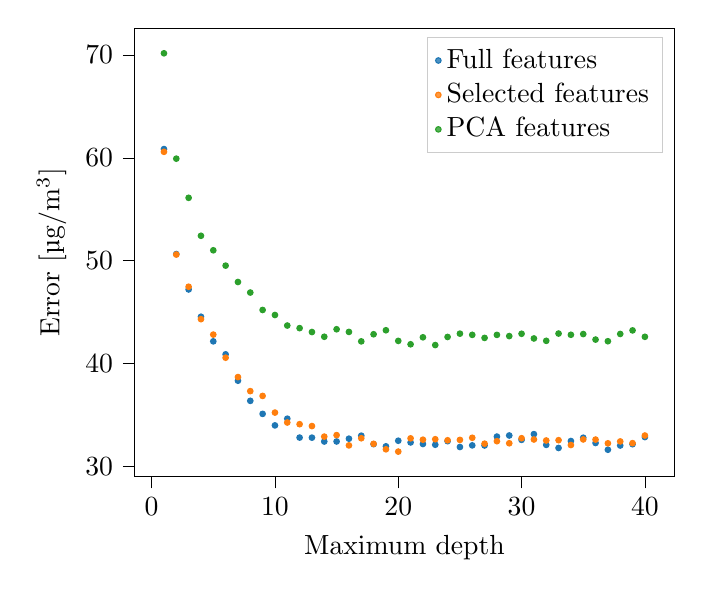
\begin{tikzpicture}

\definecolor{color0}{rgb}{0.12156862745098,0.466666666666667,0.705882352941177}
\definecolor{color1}{rgb}{1,0.498039215686275,0.0549019607843137}
\definecolor{color2}{rgb}{0.172549019607843,0.627450980392157,0.172549019607843}

\begin{axis}[
legend cell align={left},
legend style={fill opacity=0.8, draw opacity=1, text opacity=1, draw=white!80.0!black},
tick align = outside,
tick pos=left,
x grid style={white!69.01960784313725!black},
xlabel={Maximum depth},
xmin=-1.381189034867, xmax=42.381189034867,
xtick style={color=black},
y grid style={white!69.01960784313725!black},
ylabel={Error [\si{\micro g/m^3}]},
ymin=28.9946711680242, ymax=72.6087847346333,
ytick style={color=black}
]
\addplot [only marks,  mark size = 1pt, draw=color0, fill=color0, colormap/viridis]
table{%
x                      y
1 60.8516550568662
2 50.637641862368
3 47.196727851927
4 44.5422884269567
5 42.1466484920351
6 40.883523750618
7 38.3163489206734
8 36.3594383651554
9 35.0924639928978
10 33.9718938025606
11 34.6236437003025
12 32.7852331331233
13 32.780221326179
14 32.4039612793887
15 32.4075351926306
16 32.6790415417887
17 32.9706988264993
18 32.1484716702183
19 31.9355104830824
20 32.4787128506341
21 32.313635266676
22 32.1636818183206
23 32.0893400247832
24 32.4367231830001
25 31.868104170919
26 32.0289636904483
27 32.0189718090811
28 32.8828652111229
29 32.9891022387375
30 32.5650821933298
31 33.1210552433697
32 32.0755896555427
33 31.776031367133
34 32.4489405749714
35 32.7707103487006
36 32.2588927998539
37 31.603063290605
38 32.0153528774405
39 32.1420930505726
40 32.8332930724682
};
\addlegendentry{Full features}
\addplot [only marks,  mark size = 1pt, draw=color1, fill=color1, colormap/viridis]
table{%
x                      y
1 60.5857408320937
2 50.5915089120464
3 47.4612386806133
4 44.3069108138372
5 42.803064294008
6 40.5567868616982
7 38.6715135422657
8 37.3051571514534
9 36.8378505310585
10 35.2179307480805
11 34.2523121595105
12 34.0887006183638
13 33.9058491148012
14 32.8800966611186
15 33.0241847956331
16 32.0264531407759
17 32.7211777367088
18 32.1754081595169
19 31.6450191497668
20 31.4214438466759
21 32.7102260979459
22 32.5807417222717
23 32.6246119461246
24 32.5236901131248
25 32.5608548046084
26 32.767553116616
27 32.1921570970022
28 32.4338361352147
29 32.233684140503
30 32.7224852602893
31 32.6003779763632
32 32.5022591042971
33 32.5337679894024
34 32.0616151752142
35 32.604625646927
36 32.5918129750643
37 32.2286920013653
38 32.4115357928941
39 32.2456820504514
40 32.9855094933258
};
\addlegendentry{Selected features}
\addplot [only marks,  mark size = 1pt, draw=color2, fill=color2, colormap/viridis]
table{%
x                      y
1 70.1702238236892
2 59.9187505301823
3 56.1106708870888
4 52.4168878962976
5 51.0064917084385
6 49.514158730757
7 47.9209737828343
8 46.8962135957658
9 45.1994555089049
10 44.7113407156701
11 43.6858298371317
12 43.4322830879939
13 43.0539833333709
14 42.5942326865494
15 43.3238545042959
16 43.0650548351874
17 42.1461044659702
18 42.8369630022993
19 43.2274934870266
20 42.1919593550639
21 41.8618453837716
22 42.5405280958768
23 41.7864965707902
24 42.5751757101786
25 42.8965567043531
26 42.7783740585895
27 42.4819036938615
28 42.7771520244272
29 42.6582282948838
30 42.8841503902725
31 42.4287410220729
32 42.1975188963963
33 42.9061054862707
34 42.7855066311347
35 42.8564992439567
36 42.3196067080018
37 42.1598643300114
38 42.866823479395
39 43.2132996165452
40 42.5889273804234
};
\addlegendentry{PCA features}
\end{axis}

\end{tikzpicture}

    \caption{Bootstrap 632 error for the Bagging trees model}
    \label{fig:boost_tree}
\end{figure}

\subsection{Multilayer Perceptron}

A multilayer perceptron takes as inputs the features (17 for the full set and 7 for the selected/PCA set) and propagates these information though a deep neural network to output the final PM2.5 estimation. At each layer, the data are subject to a batch normalisation followed by a ReLU activation function.

Considering the high number of parameters which are subject to optimization (number of hidden layers, neurons per hidden layer, epochs, learning rate, batch size), it might seem interesting to use an optimization algorithm such as a greedy search or a genetic search. However, it appears after simulation that finding this optimum is difficult since the performances are better when the network is very large, in such a way that overfitting is only noticed for big neural networks which are impossible to train in a limited time. The following paragraphs will thus be dedicated to analysing the error for several numbers of neurons per layer, epochs per training period, and hidden layers.

The results presented in Figure~\ref{fig:MLP} depict the error variation for different numbers of neurons (hyperparameter) in each of the 8 hidden layers, ranging from 1 to 50. The learning step is done by feeding the network with the inputs/output pairs, more precisely with 50 epochs and a batch size of 128. It can be seen that the neural network performs the best with the full features as inputs since the weights of the network are precisely adapted to select the information in each features, even the smallest one. On the other hand, deep neural networks do not aim at dropping some features, which is proven by the poor results from features selection and features extraction.

\begin{figure}[H]
    \centering
    % This file was created by tikzplotlib v0.8.7.
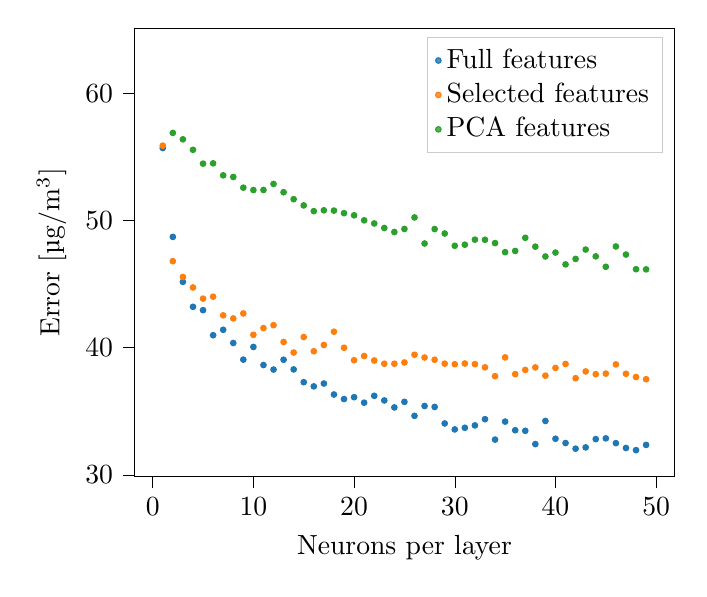
\begin{tikzpicture}

\definecolor{color0}{rgb}{0.12156862745098,0.466666666666667,0.705882352941177}
\definecolor{color1}{rgb}{1,0.498039215686275,0.0549019607843137}
\definecolor{color2}{rgb}{0.172549019607843,0.627450980392157,0.172549019607843}

\begin{axis}[
legend cell align={left},
legend style={fill opacity=0.8, draw opacity=1, text opacity=1, draw=white!80.0!black},
tick align=outside,
tick pos=left,
x grid style={white!69.01960784313725!black},
xlabel={Neurons per layer},
xmin=-1.79609509496988, xmax=51.7960950949699,
xtick style={color=black},
y grid style={white!69.01960784313725!black},
ylabel={Error [\si{\micro g/m^3}]},
ymin=29.8695621095969, ymax=65.1164340378912,
ytick style={color=black}
]
\addplot [only marks, mark size=1pt, draw=color0, fill=color0, colormap/viridis]
table{%
x                      y
1 55.6950910071091
2 48.711203721216
3 45.1729350213493
4 43.2118633834967
5 42.9499941573174
6 40.9790839555033
7 41.4055482827309
8 40.368838273728
9 39.061165974862
10 40.0571003231887
11 38.6369453410261
12 38.2795251798468
13 39.0520677302609
14 38.2920215098749
15 37.2898673484965
16 36.9580541531945
17 37.1837110059168
18 36.3184736190567
19 35.9613202502897
20 36.1087143336349
21 35.6771070079794
22 36.2140046395798
23 35.8528430537507
24 35.3039715450485
25 35.7403751377403
26 34.640761379515
27 35.4163487152852
28 35.340913944067
29 34.0431726235607
30 33.5742655366986
31 33.7028479010602
32 33.8904895600423
33 34.3780908727686
34 32.773662162134
35 34.1888448707388
36 33.5088496694488
37 33.4645263303908
38 32.42088331374
39 34.2394565058546
40 32.841114640961
41 32.5030807552868
42 32.06158188129
43 32.1614182809041
44 32.8123769156681
45 32.8709488317845
46 32.4950311360459
47 32.1132106563761
48 31.9445269550899
49 32.3565888091737
};
\addlegendentry{Full features}
\addplot [only marks, mark size = 1pt, draw=color1, fill=color1, colormap/viridis]
table{%
x                      y
1 55.8844511849768
2 46.802636677314
3 45.5596016459429
4 44.7350839639823
5 43.8576225377128
6 44.0111936529671
7 42.5429902077742
8 42.3011027925133
9 42.690752609739
10 41.0116703889277
11 41.542108899876
12 41.7705003450155
13 40.4495879429057
14 39.6188981669241
15 40.8334847001448
16 39.7204446215047
17 40.2149889150813
18 41.2569528707066
19 39.9938611200442
20 39.0146620752818
21 39.3430828751147
22 38.9917232488845
23 38.7397003659709
24 38.7392530200791
25 38.8385101718314
26 39.4431627038594
27 39.2289317341698
28 39.0525815473667
29 38.7445580087351
30 38.7007366236285
31 38.7560607190231
32 38.7069796723287
33 38.4545433216958
34 37.7606826596415
35 39.2349762438926
36 37.9205539185357
37 38.2534468105952
38 38.4487594153359
39 37.8006267522299
40 38.4100679761512
41 38.7224955137855
42 37.6037938089892
43 38.1319328032114
44 37.918503379306
45 37.9626880153008
46 38.6870862151597
47 37.9498140045176
48 37.6937652394231
49 37.5199160112602
};
\addlegendentry{Selected features}
\addplot [only marks, mark size = 1pt, draw=color2, fill=color2, colormap/viridis]
table{%
x                      y
1 69.0059230997545
2 56.8854535960351
3 56.3800917166031
4 55.5564681291941
5 54.4689601772195
6 54.4926189632234
7 53.5481484557598
8 53.420356863532
9 52.5801632074563
10 52.3932360038491
11 52.3980650623564
12 52.8730580785524
13 52.2210600910031
14 51.6743589776825
15 51.1870986123949
16 50.736481436438
17 50.8004734422654
18 50.778129249398
19 50.576054506019
20 50.4070742138456
21 50.0145203031037
22 49.7671661391319
23 49.4114603925856
24 49.0931107477781
25 49.3306050308477
26 50.2399176684445
27 48.1904527022729
28 49.3275636521116
29 48.9771737877655
30 48.0120377406641
31 48.0968465905423
32 48.4953840445801
33 48.4825313294269
34 48.222288036082
35 47.5100110980396
36 47.6062630410809
37 48.639356139655
38 47.942433636644
39 47.1710937160557
40 47.4797208932187
41 46.549799813657
42 46.978007583421
43 47.7156298421343
44 47.1795954388903
45 46.3597158093353
46 47.9565867379474
47 47.3227923459689
48 46.1708425801179
49 46.156654311703
};
\addlegendentry{PCA features}
\end{axis}

\end{tikzpicture}

    \caption{Bootstrap 632 error for the MLP model with different numbers of neurons per hidden layer}
    \label{fig:MLP}
\end{figure}

One can also analyse the error for different training periods, characterised by a varying number of epochs. Figure~\ref{fig:MLP_epochs} shows this error with a number of epochs ranging from 1 to 80. The error is stabilized after around 50 epochs for all inputs subsets since all the neural networks weights do not vary anymore. The error does not increase for additional epochs, leading to the conclusion that the network configuration is too small to bring overfitting due to long training periods\footnote{In case of possible overfitting, the early stop approach consists to stop the training when the validation error reaches a minimum.}.

\begin{figure}[H]
    \centering
    % This file was created by tikzplotlib v0.8.7.
\begin{tikzpicture}

\definecolor{color0}{rgb}{0.12156862745098,0.466666666666667,0.705882352941177}
\definecolor{color1}{rgb}{1,0.498039215686275,0.0549019607843137}
\definecolor{color2}{rgb}{0.172549019607843,0.627450980392157,0.172549019607843}

\begin{axis}[
legend cell align={left},
legend style={fill opacity=0.8, draw opacity=1, text opacity=1, draw=white!80.0!black},
tick align=outside,
tick pos=left,
x grid style={white!69.01960784313725!black},
xlabel={epochs},
xmin=-3.60190546683368, xmax=84.6019054668337,
xtick style={color=black},
y grid style={white!69.01960784313725!black},
ylabel={Error [ug/m\^3]},
ymin=30.8655586235403, ymax=62.4974328045426,
ytick style={color=black}
]
\addplot [only marks, marker=*, draw=color0, fill=color0, colormap/viridis]
table{%
x                      y
1 49.4386248645095
2 43.8165147846147
3 42.5410126451546
4 40.5520631836332
5 41.178450931352
6 40.5861658989833
7 38.9198028973063
8 38.7517448288748
9 38.4731717625789
10 38.5998005332223
11 37.4011359089472
12 38.3428946005182
13 37.6224905214733
14 37.413186135286
15 36.9657819270586
16 36.8751445395673
17 36.3899067414357
18 35.8289621883778
19 36.7437935426603
20 36.6603571778592
21 36.1786930673779
22 36.2887728355504
23 35.0886895254477
24 36.1734799672468
25 35.76403138549
26 35.2602394481911
27 35.4937500908337
28 35.8380074648475
29 36.3002584852843
30 35.2868800230522
31 34.6169602015756
32 34.4232833456155
33 33.9413579520519
34 34.4204705440865
35 34.941410916782
36 34.5251312469016
37 34.0591935380518
38 33.7646281923352
39 33.6490736540941
40 34.3018563193482
41 34.523532373609
42 33.9349492309351
43 33.7957886045292
44 33.8708768401956
45 33.9694870225764
46 33.9370965892054
47 33.8977942615851
48 33.6643309786526
49 33.7719613542671
50 33.6917137546688
51 33.4724968147663
52 33.0586396616781
53 33.2720457863299
54 33.9595520400896
55 34.0480990180241
56 34.2182266786759
57 34.0205292014834
58 33.8129197273707
59 33.3491925308087
60 33.447156845932
61 32.3414554586187
62 33.012033359743
63 33.4182525258072
64 33.8619068686574
65 33.3175602675248
66 34.0034167467315
67 32.9649058716004
68 32.5934846764411
69 33.5720470013822
70 33.2114237405344
71 32.6824090687534
72 33.1627165310724
73 33.000823544263
74 32.6164909531792
75 33.3017440845272
76 32.4149458148821
77 33.0881983662595
78 33.0581560586364
79 33.3458421084542
80 32.3125690259747
};
\addlegendentry{Full features}
\addplot [only marks, marker=*, draw=color1, fill=color1, colormap/viridis]
table{%
x                      y
1 51.8229815310347
2 46.766492672185
3 45.468151344409
4 45.7694956848013
5 44.8270874440802
6 44.5203976341303
7 44.3099451241266
8 43.1967151318243
9 43.0257876122312
10 43.1767833799425
11 42.928181802953
12 43.4542010263643
13 43.1471483901594
14 42.9960078616937
15 42.2408933630605
16 42.2000996956
17 42.795682817753
18 41.7370492165141
19 42.3910895745221
20 41.4212142950113
21 41.7373950172776
22 43.0615339865076
23 41.180026454128
24 41.1646297370151
25 41.3139358023105
26 41.7410392587655
27 41.1984030308924
28 41.2529367152039
29 41.0977518278958
30 41.0871710883681
31 40.823150047319
32 40.3764743341515
33 40.6052173291355
34 40.6493432717145
35 39.5727579644491
36 40.7458373600855
37 40.3819900497242
38 40.2965810748355
39 41.4287253047798
40 40.1898606490285
41 40.8371287707468
42 40.8961452993637
43 39.4595958028027
44 40.3595392940703
45 39.838363849704
46 39.7058206421049
47 39.7280584402189
48 40.4697759289497
49 38.9777031712217
50 39.647907128845
51 40.3080094367206
52 39.1259981934069
53 38.4334001037798
54 40.1248424922513
55 39.2474270583868
56 38.8736368378427
57 39.4800359464948
58 38.8759179814911
59 39.1576384015683
60 38.3939239698038
61 40.2527918117957
62 39.1816953275572
63 39.4542201377223
64 39.072789634646
65 39.1112367076577
66 38.3046606882351
67 39.228099158045
68 38.6452398497502
69 39.2031539985728
70 39.4720312151548
71 37.5474979761247
72 38.2064171955142
73 38.5569193565015
74 38.2893791033824
75 38.8827245987092
76 38.5037062741678
77 38.4975055184619
78 38.7926612050572
79 38.3851344132529
80 38.6927834463747
};
\addlegendentry{Selected features}
\addplot [only marks, marker=*, draw=color2, fill=color2, colormap/viridis]
table{%
x                      y
1 60.8603710703897
2 56.5928488728036
3 56.4173002094357
4 55.6431722271604
5 55.6401851233066
6 54.1917411147446
7 54.6691422661879
8 54.2175908744828
9 54.3833442328246
10 53.3020217622666
11 53.175577248982
12 52.819666064327
13 52.8604406151759
14 52.528341198147
15 52.3077911365731
16 52.1672967791374
17 52.2283111780186
18 52.2296177317348
19 52.2116828805834
20 51.1387558385865
21 51.3136425370193
22 51.5582765892864
23 51.0972446015694
24 51.3851114425632
25 50.1620144783245
26 50.7562718009209
27 51.0639762361933
28 49.6619529395263
29 50.2031370589653
30 49.146485184655
31 49.8186426392797
32 50.3126972242353
33 49.7130147331555
34 49.4414871422234
35 48.7956989560249
36 48.8258200376381
37 49.3844313685212
38 48.6092221524897
39 48.8530018336165
40 48.9061165463714
41 49.4594523172916
42 48.3606752080592
43 49.9425820513033
44 48.0986598149955
45 48.0986598149955
46 49.1883556337766
47 49.2485877102333
48 48.1403223593278
49 48.4404567588238
50 47.693300923889
51 48.6848281662175
52 48.5579456820926
53 48.1918279742542
54 48.3351047442726
55 47.707226864977
56 48.1403190124252
57 48.6228527436181
58 47.0885830816534
59 47.5841615482059
60 47.6129525666745
61 47.1160636145789
62 47.954400466045
63 47.5714784715485
64 46.8774869655175
65 47.0667373698578
66 46.1220728537033
67 47.2174647208666
68 47.019519324701
69 47.111652485112
70 47.7110341507103
71 46.8513731380808
72 47.7333479740901
73 46.3678195349074
74 47.6440538855377
75 47.1344752111205
76 46.9327909298104
77 46.8606884396839
78 46.1449826775943
79 46.9154630871431
80 47.182605148656
};
\addlegendentry{PCA features}
\end{axis}

\end{tikzpicture}

    \caption{Bootstrap 632 error for the MLP model with different numbers of epochs per training period}
    \label{fig:MLP_epochs}
\end{figure}

The next step thus consists to increase the number of hidden layers and reduce the error as far as possible. Figure~\ref{fig:MLP_layers} presents this error for the full set, 50 neurons per hidden layer and a number of epochs proportional to the number of layers since larger networks require a longer training period. One can see a minimum error for 18 hidden layers but no overfitting appears as it should be expected for such large networks. Hence, overfitting should arise for larger networks.

\begin{figure}[H]
    \centering
    % This file was created by tikzplotlib v0.8.7.
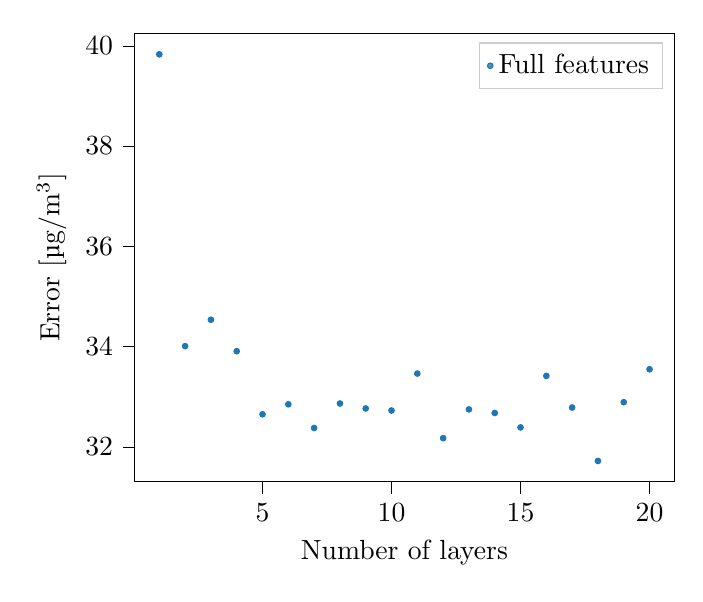
\begin{tikzpicture}

\definecolor{color0}{rgb}{0.12156862745098,0.466666666666667,0.705882352941177}

\begin{axis}[
legend cell align={left},
legend style={fill opacity=0.8, draw opacity=1, text opacity=1, draw=white!80.0!black},
tick align=outside,
tick pos=left,
x grid style={white!69.01960784313725!black},
xlabel={Number of layers},
xmin=0.0426075268817202, xmax=20.9573924731183,
xtick style={color=black},
y grid style={white!69.01960784313725!black},
ylabel={Error [\si{\micro g/m^3}]},
ymin=31.3018482631426, ymax=40.2457384004481,
ytick style={color=black}
]
\addplot [only marks, mark size = 1pt, draw=color0, fill=color0, colormap/viridis]
table{%
x                      y
1 39.83
2 34.0080525997711
3 34.5349886207359
4 33.907052887754
5 32.6486946971239
6 32.848148954324
7 32.3750906378598
8 32.8638097894373
9 32.7653191574057
10 32.7239935610875
11 33.4613292552297
12 32.1726450762728
13 32.7460092811903
14 32.6746261177239
15 32.3869844118639
16 33.4143275178886
17 32.7837407020655
18 31.7175866635907
19 32.8903746936802
20 33.546754434564
};
\addlegendentry{Full features}
\end{axis}

\end{tikzpicture}

    \caption{Bootstrap 632 error for the MLP model with different numbers of hidden layers}
    \label{fig:MLP_layers}
\end{figure}

Finally, a huge neural network of 20 hidden layers and 100 neurons has been trained with 300 epochs. It gives a bootstrap 632 error of \SI{34.12}{\micro g/m^3}, suggesting the start of a small overfitting.

It can be noted that the PyTorch library has been used, leading the authors to implement an estimator in order to match the specifications of the bootstrap 632 method \cite{NEURIPS2019_9015}.

\section{Conclusion}
\label{Conclusion}

To conclude, the lowest error for the analysed models are summarized in Table~\ref{tab:sum} (the errors are expressed in \si{\micro g/m^3}).

\begin{table}[H]
\setlength\abovecaptionskip{-2\baselineskip}
\centering
\begin{tabular}{lccc}
\hline
 Model &  Error (Full) &  Error (Selected) &  Error (PCA)\\ \hline
 Linear regression & 44.35 & 44.50 & 54.10 \\
 Ridge regression & 44.15 & 44.38 & 53.91  \\ 
 Lasso & 44.06 & 44.07 & 53.92 \\
 KNN & 44.12 & 38.51 & 48.58 \\
 Regression tree & 40.39 & 40.23 & 51.48 \\
 Boot. agg. trees & 31.60 & 31.42 & 41.78 \\
 MLP & 31.94 & 37.52 & 46.16 \\ \hline
\end{tabular}
\vspace*{3mm}
\caption{Summarized error for all the models}
\label{tab:sum}
\end{table}

\subsection{Final model selection}

The bootstrap aggregating trees method with the features selection is chosen as the final method since it has the lowest error. This model is used to predict the output of the secret set, \texttt{Y2}. The bootstrap 632 method aims to estimate the error on a set belonging to the entire possible space. Hence, the expected RMS error on \texttt{Y2} is the bootstrap 632 error on \texttt{Y1}: \SI{31.42}{\micro g/m^3}.

Finally, combining the previous model predictions by means of ensemble methods or a voting classifier are good perspectives for a future work in the prediction improvements and the quest for the lowest error.

\printbibliography

\end{document}
